\documentclass{jsarticle}
\usepackage{color}
\usepackage{bm}
\usepackage{mathrsfs}
\usepackage[height=26cm,width=16cm]{geometry} 
\usepackage{amsmath}
\usepackage{cases}
\usepackage[dvipdfmx]{graphicx}
\title{力学2}
\graphicspath{{./image/}}

\begin{document}

\section{Prblm2}
	\begin{center}
		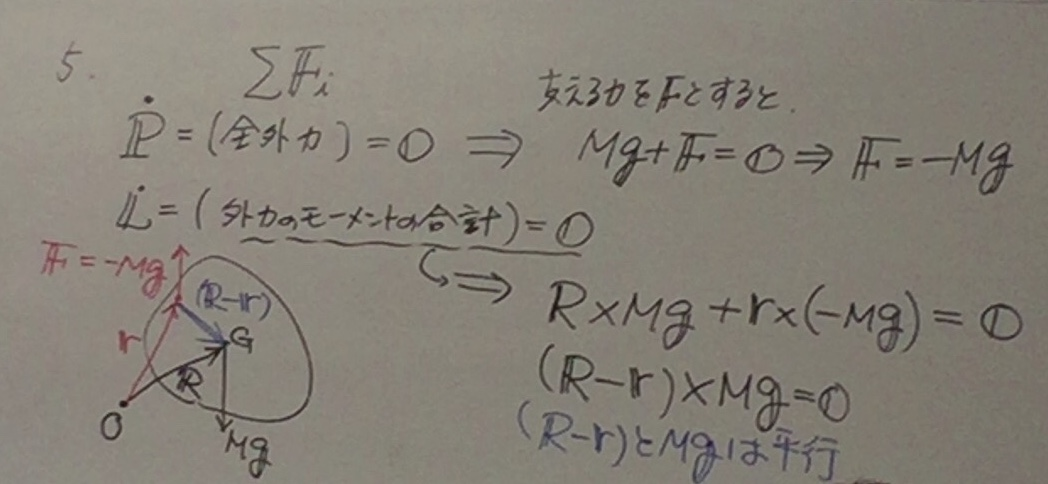
\includegraphics[width=12cm]{5_13_1.JPG}
	\end{center}
	\begin{center}
		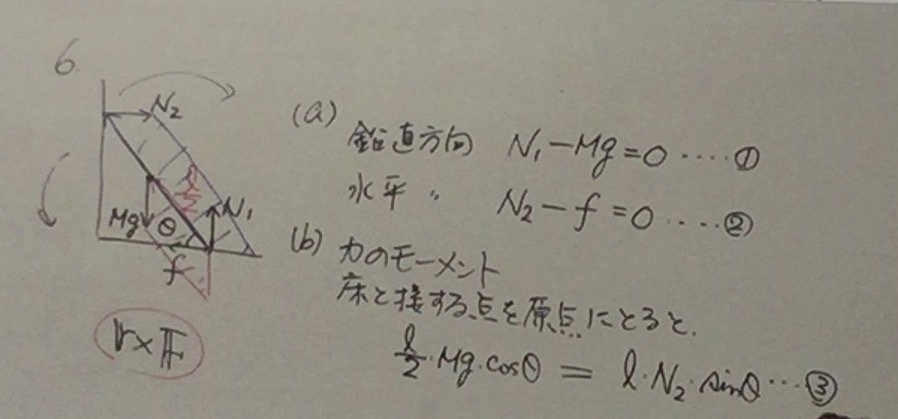
\includegraphics[width=12cm]{5_13_2.JPG}
	\end{center}
	\begin{center}
		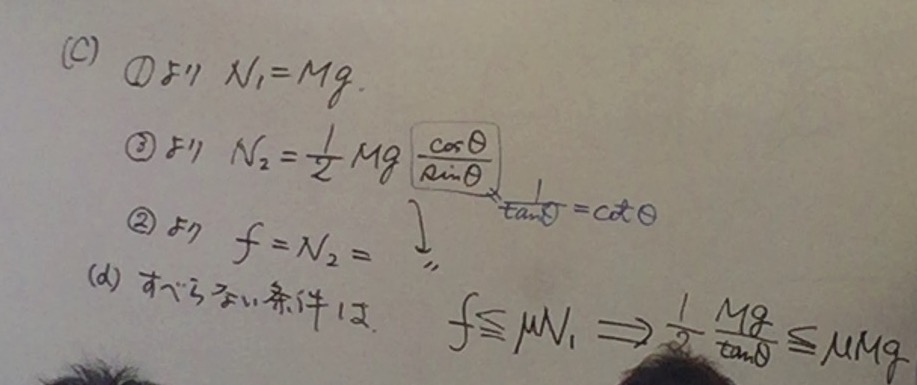
\includegraphics[width=12cm]{5_13_3.JPG}
	\end{center}
	\begin{center}
		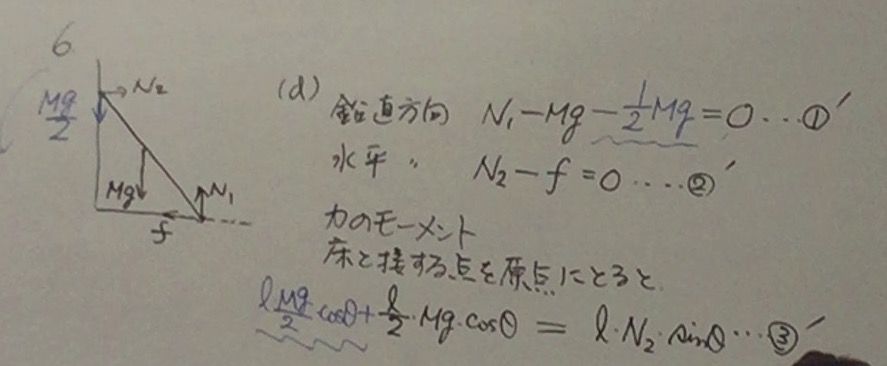
\includegraphics[width=12cm]{5_13_4.JPG}
	\end{center}
	\begin{center}
		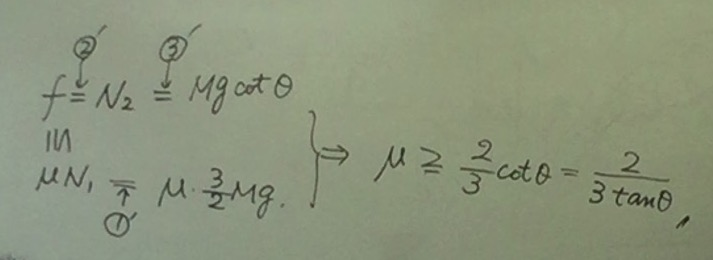
\includegraphics[width=12cm]{5_13_5.JPG}
	\end{center}
	\begin{center}
		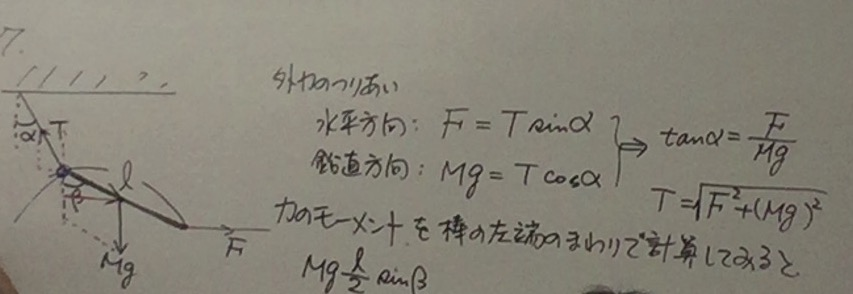
\includegraphics[width=12cm]{5_13_6.JPG}
	\end{center}
	
\section{Prblm3}
	\begin{center}
		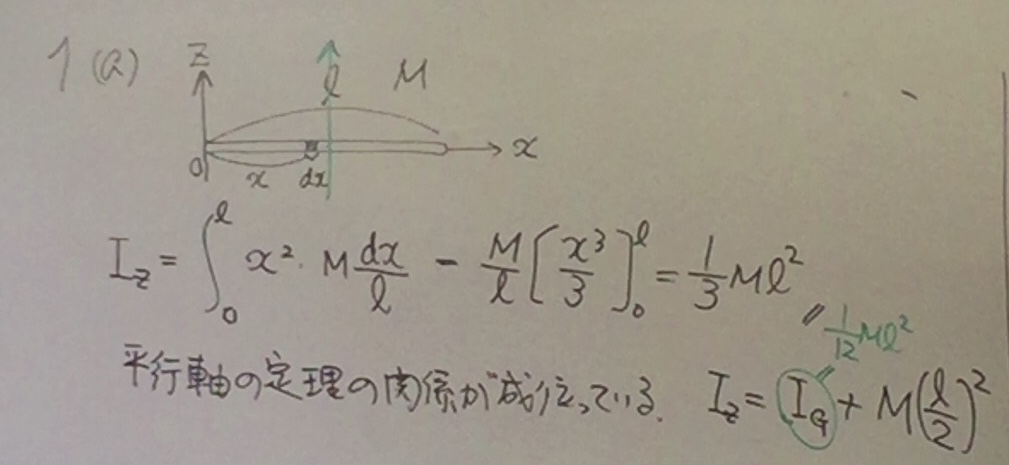
\includegraphics[width=12cm]{5_20_1.JPG}
	\end{center}
	\begin{center}
		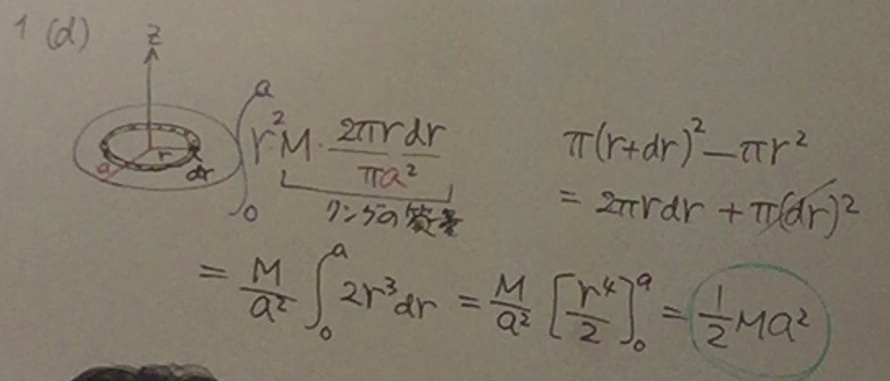
\includegraphics[width=12cm]{5_20_2.JPG}
	\end{center}
	\begin{center}
		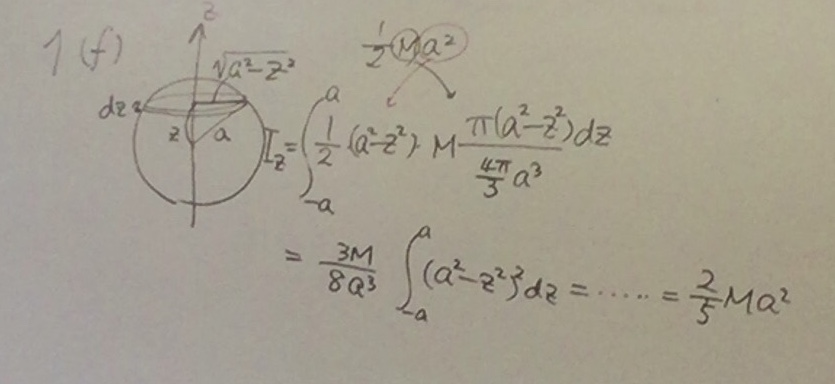
\includegraphics[width=12cm]{5_20_3.JPG}
	\end{center}
	\begin{center}
		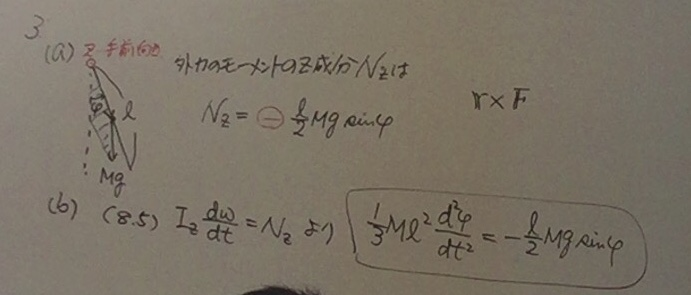
\includegraphics[width=12cm]{5_20_4.JPG}
	\end{center}
	\begin{center}
		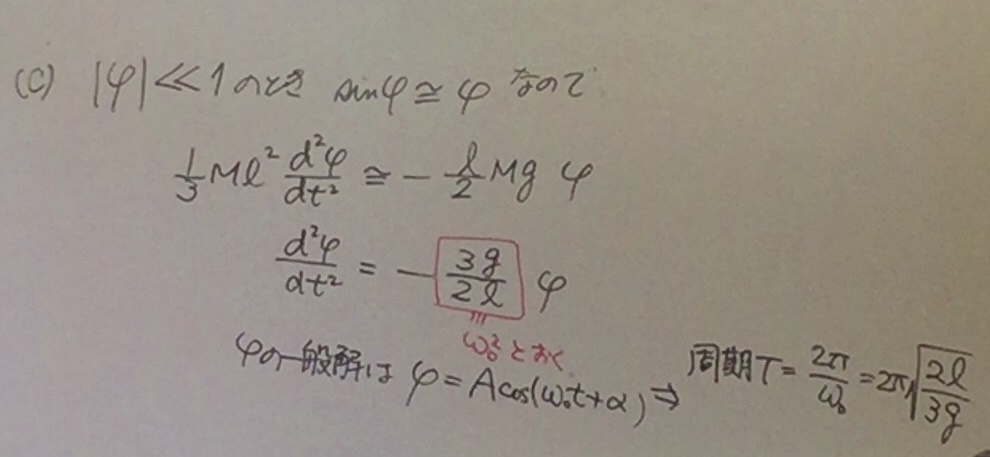
\includegraphics[width=12cm]{5_20_5.JPG}
	\end{center}
	\begin{center}
		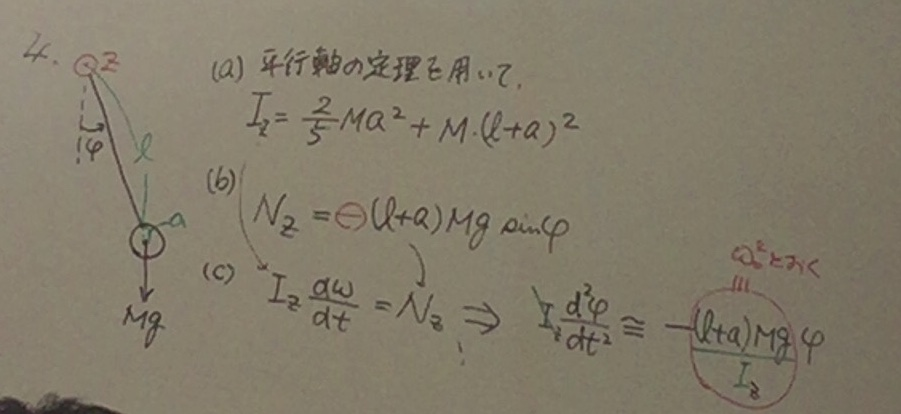
\includegraphics[width=12cm]{5_20_6.JPG}
	\end{center}
	
\section{Prblm3}
	\begin{center}
		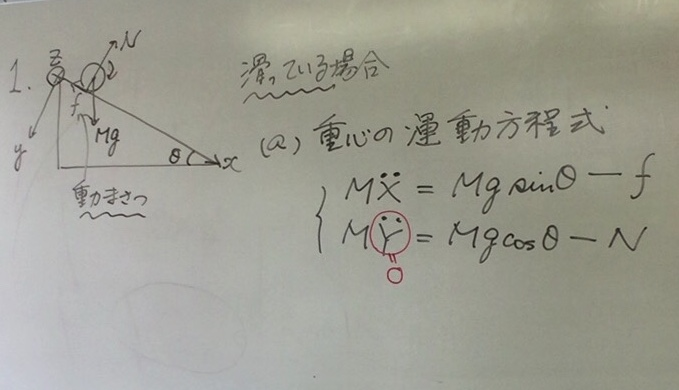
\includegraphics[width=12cm]{5_27_1.JPG}
	\end{center}
	\begin{center}
		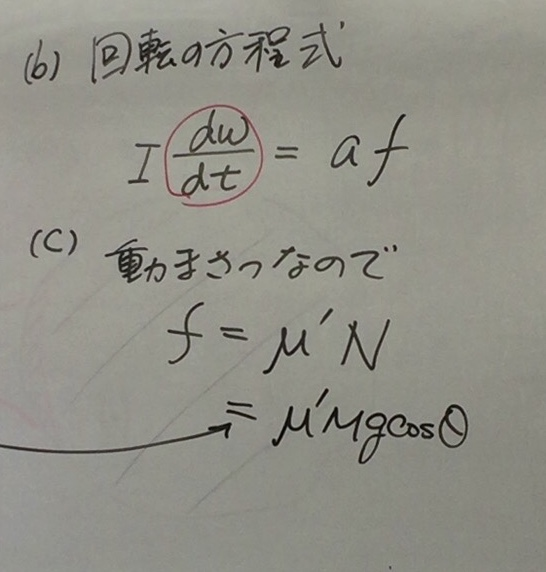
\includegraphics[width=12cm]{5_27_2.JPG}
	\end{center}
	\begin{center}
		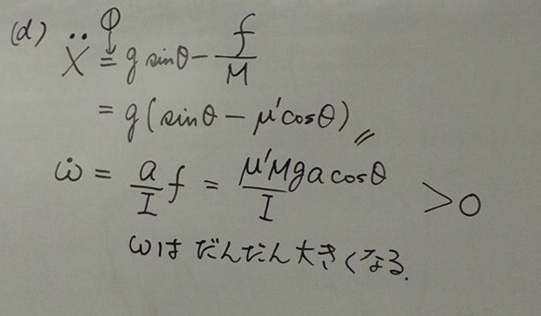
\includegraphics[width=12cm]{5_27_3.JPG}
	\end{center}
	\begin{center}
		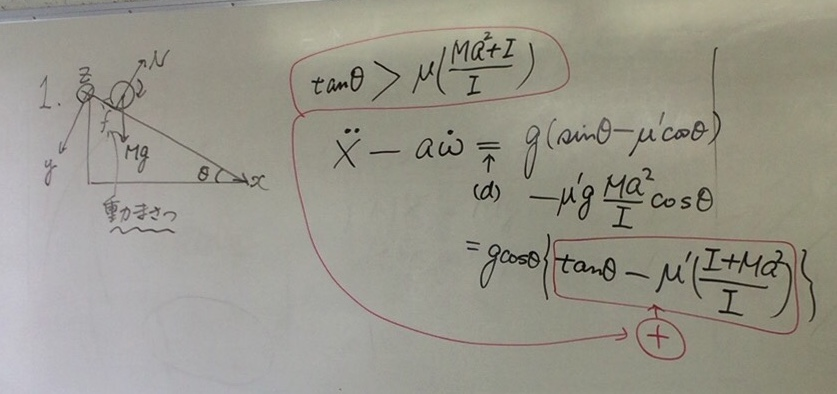
\includegraphics[width=12cm]{5_27_4.JPG}
	\end{center}
	\begin{center}
		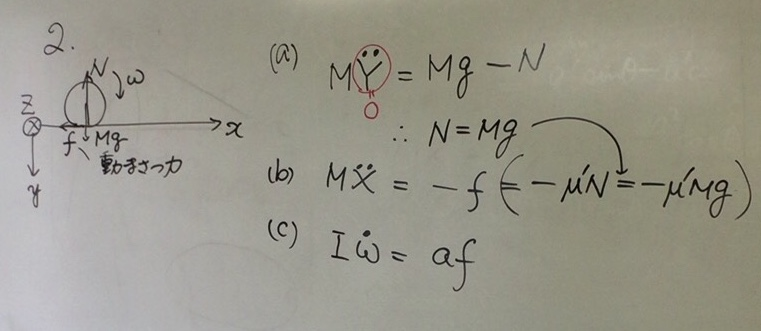
\includegraphics[width=12cm]{5_27_5.JPG}
	\end{center}
	\begin{center}
		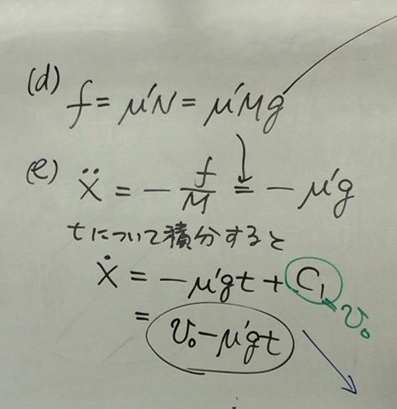
\includegraphics[width=12cm]{5_27_6.JPG}
	\end{center}
	\begin{center}
		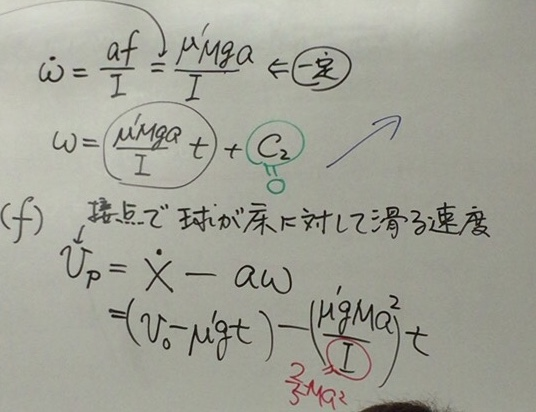
\includegraphics[width=12cm]{5_27_7.JPG}
	\end{center}
	\begin{center}
		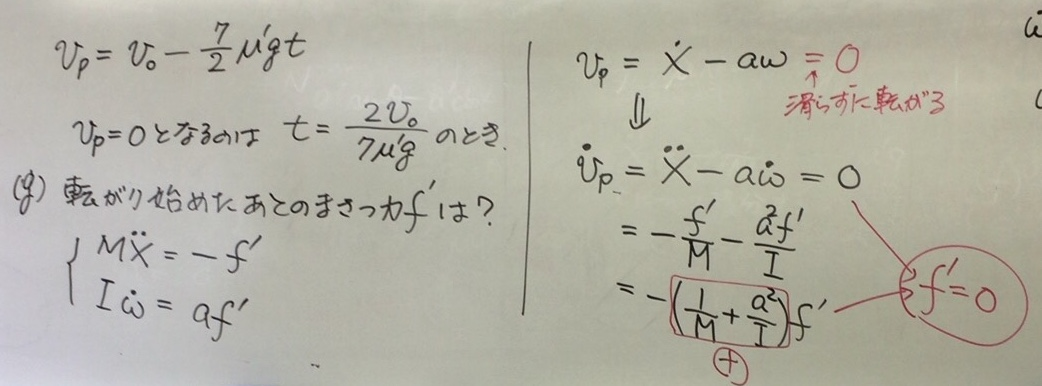
\includegraphics[width=12cm]{5_27_8.JPG}
	\end{center}
	\begin{center}
		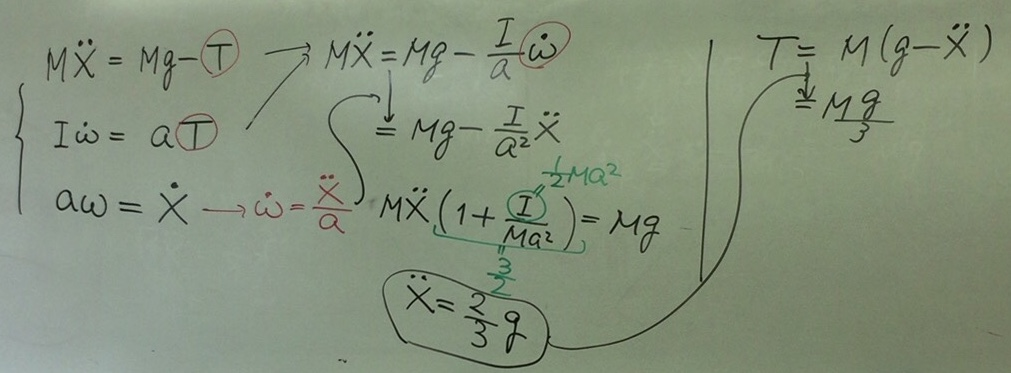
\includegraphics[width=12cm]{5_27_9.JPG}
	\end{center}




\end{document}